\documentclass{standalone}
\usepackage{tikz}

\begin{document}
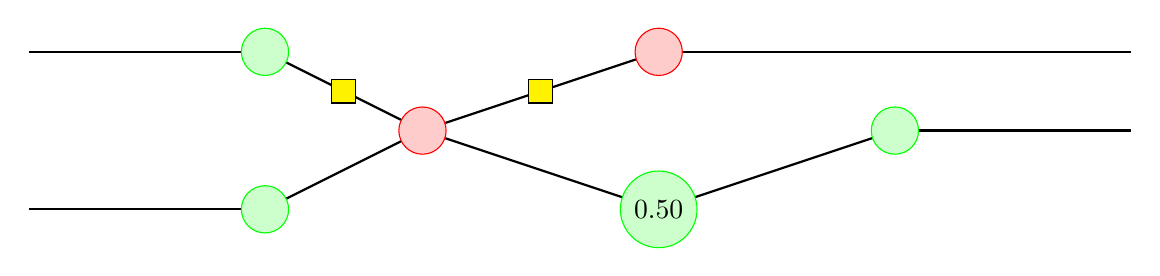
\begin{tikzpicture}[
    z_node/.style={circle,draw=green,fill=green!20,minimum size=6mm,text=black},
    x_node/.style={circle,draw=red,fill=red!20,minimum size=6mm,text=black},
    regular_edge/.style={black,thick},
    hadamard_edge/.style={black,thick},
    hadamard_box/.style={fill=yellow,draw=black,minimum size=3mm},
    small_hadamard_box/.style={fill=yellow,draw=black,minimum size=2mm},
    edge_count/.style={text=black,font=\scriptsize},
    input_wire/.style={thick,black},
    output_wire/.style={thick,black}]
  \draw[input_wire] (-7.00,1.00) -- (-4.00,1.00);
  \draw[input_wire] (-7.00,-1.00) -- (-4.00,-1.00);
  \draw[output_wire] (1.00,1.00) -- (7.00,1.00);
  \draw[output_wire] (4.00,0.00) -- (7.00,0.00);
\node[z_node] (0) at (-4.00,-1.00) {};
\node[z_node] (1) at (-4.00,1.00) {};
\node[x_node] (2) at (-2.00,0.00) {};
\node[z_node] (3) at (1.00,-1.00) {0.50};
\node[z_node] (4) at (4.00,0.00) {};
\node[x_node] (5) at (1.00,1.00) {};
\draw[regular_edge] (0) .. controls (-3.40,-0.70) and (-2.60,-0.30) .. (2);
\draw[hadamard_edge] (1) .. controls (-3.40,0.70) and (-2.60,0.30) .. (2);
\node[hadamard_box] (h1) at (-3.00,0.50) {};
\draw[regular_edge] (2) .. controls (-1.10,-0.30) and (0.10,-0.70) .. (3);
\draw[hadamard_edge] (2) .. controls (-1.10,0.30) and (0.10,0.70) .. (5);
\node[hadamard_box] (h4) at (-0.50,0.50) {};
\draw[regular_edge] (3) .. controls (1.90,-0.70) and (3.10,-0.30) .. (4);
\end{tikzpicture}
\end{document}
